\documentclass[9pt]{beamer}
%\usetheme[background=light]{metropolis}
\usetheme{Copenhagen}
\usecolortheme{seagull}
%\setmonofont{Ubuntu Mono}

\usepackage[utf8]{inputenc}

\title{Software Engineering(SE) Daily}
\subtitle{a Audio Podcast App for Software Community}
\author{Rihan Stephen Pereira \& Niranjan Pawar }
\institute[California State University, Channel Islands]
{
  %\inst{1}%
  COMP 590 - Android Development, Fall 2018\\
  Department of Computer Science\\
  California State University, Channel Islands
}
\date{\today}

% Delete this, if you do not want the table of contents to pop up at
% the beginning of each subsection:
%\AtBeginSubsection[]
%{
%  \begin{frame}<beamer>{Outline}
%    \tableofcontents[currentsection,currentsubsection]
%  \end{frame}
%}

\begin{document}

% title frame, marks the beginning of presentation
\begin{frame}[plain]
  \frametitle{}
  \titlepage
\end{frame}

% table of contents a.k.a outline
\begin{frame}[plain]
  \frametitle{Discussion}
  \tableofcontents
\end{frame}

% real meat of the presentation
% -------------------------------------

\section{Background}
\begin{frame}{Background}
  \begin{itemize}
  \item produces technical content on variety of software engineering topics
    \pause
  \item  open source project - \href{https://github.com/SoftwareEngineeringDaily}{https://github.com/SoftwareEngineeringDaily}
    \pause
  \item monthly active users, roughly 50
    \pause
  \item available on web, android and IOS
  \end{itemize}
\end{frame}


% -------------------------------------

\section{Architecture}
\begin{frame}{Architecture(System Diagram)}
  \centering{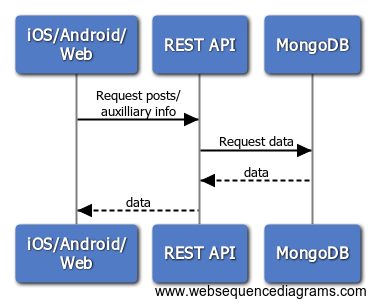
\includegraphics[width=80mm, height=60mm, scale=0.1]{img/system_diagram.png}}
\end{frame}

% -------------------------------------

\begin{frame}{a note on data miner}
  \centering{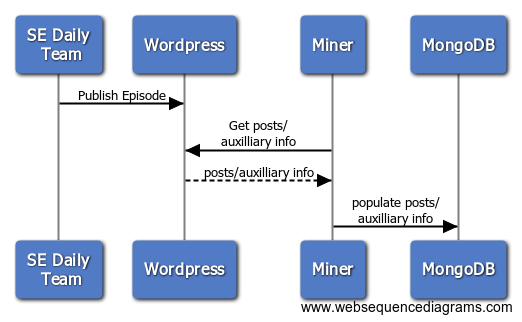
\includegraphics[width=90mm, height=50mm, scale=0.1]{img/data_miner.png}}
\end{frame}

% -------------------------------------

\section{SE-Daily Android}
\begin{frame}{SE-Daily Android Design}
  \begin{columns}
    \column{0.5\textwidth}
    \centering{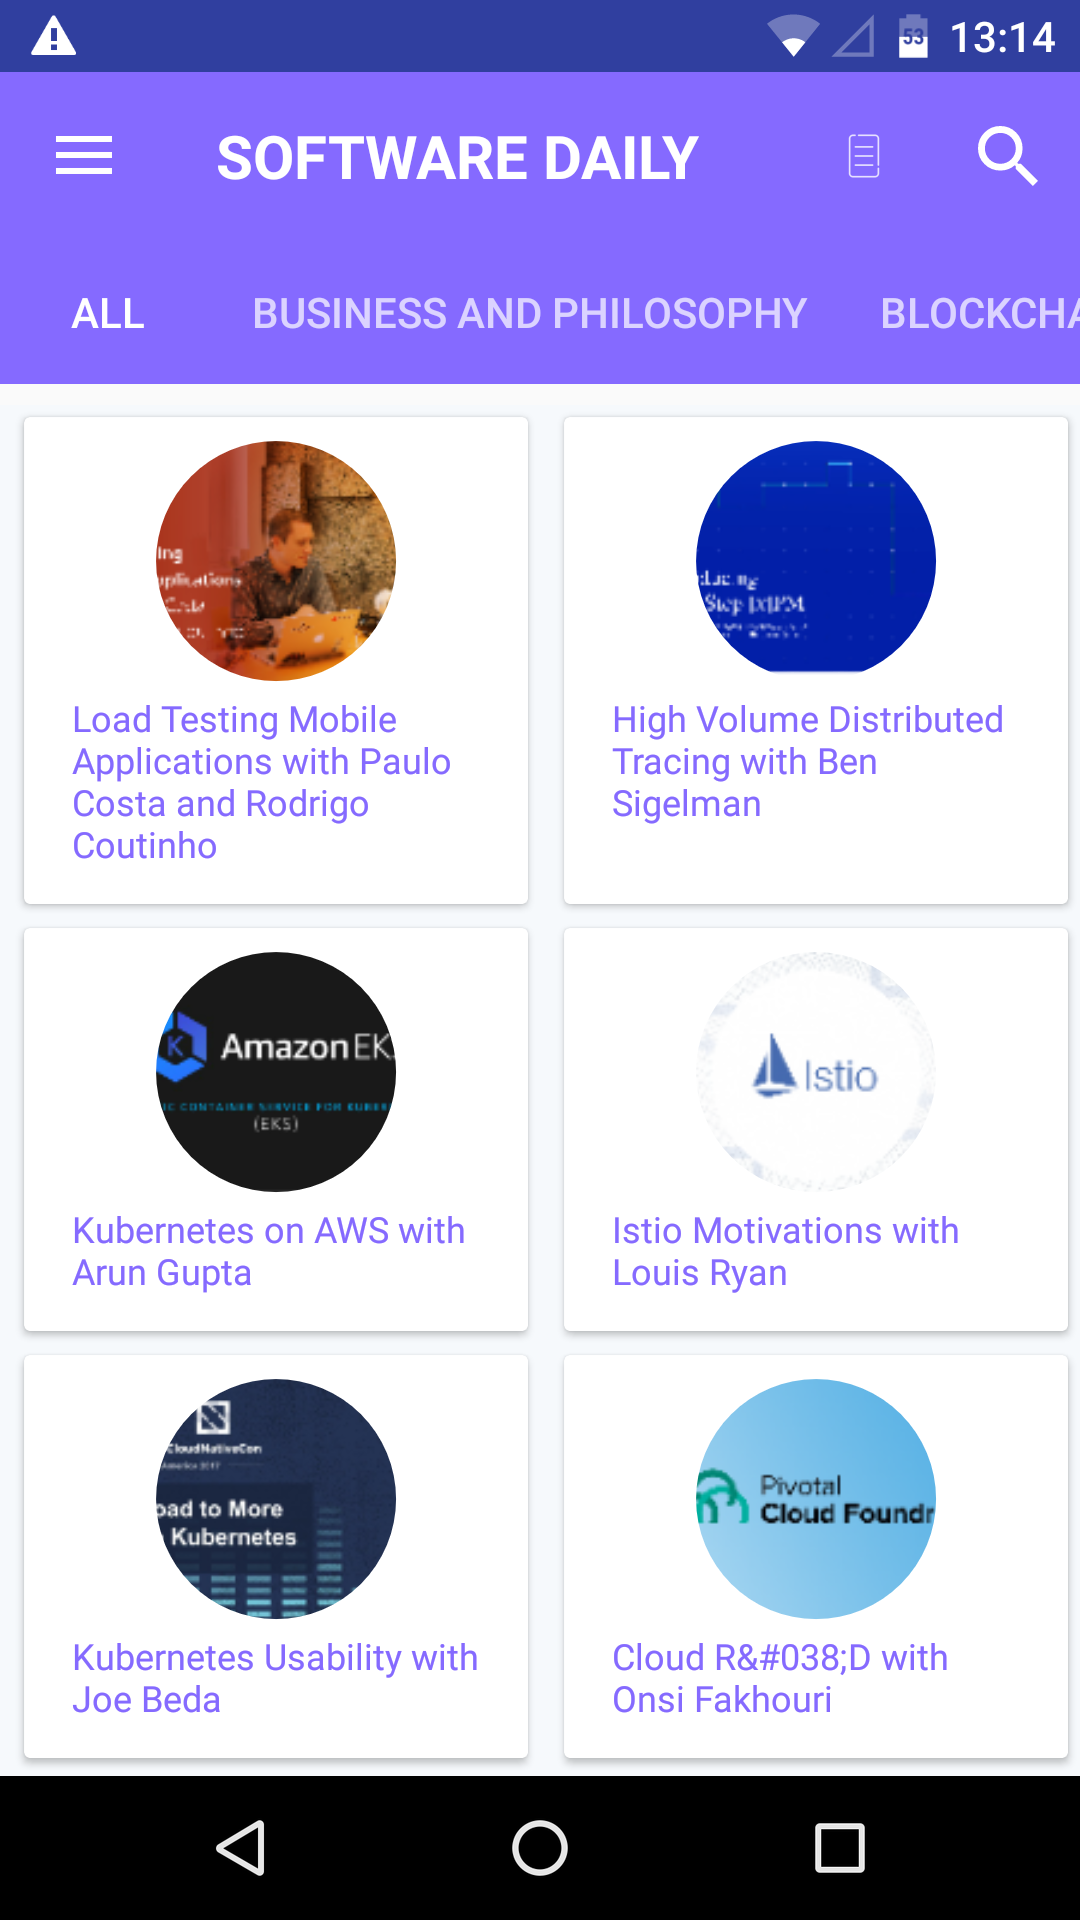
\includegraphics[width=40mm, height=70mm, scale=0.1]{img/main.png}}
    \column{0.5\textwidth}
    \begin{itemize}
    \item uses google material UI
      \pause
    \item main activity consists of top toolbar, view pager category, and fragments tied to categories
    \end{itemize}
  \end{columns}
\end{frame}

% -------------------------------------

\subsection{feature 1 - List/Grid View Toggle}
\begin{frame}{feature 1 - List/Grid View Toggle}
  \begin{columns}
    \column{0.5\textwidth}
    \centering{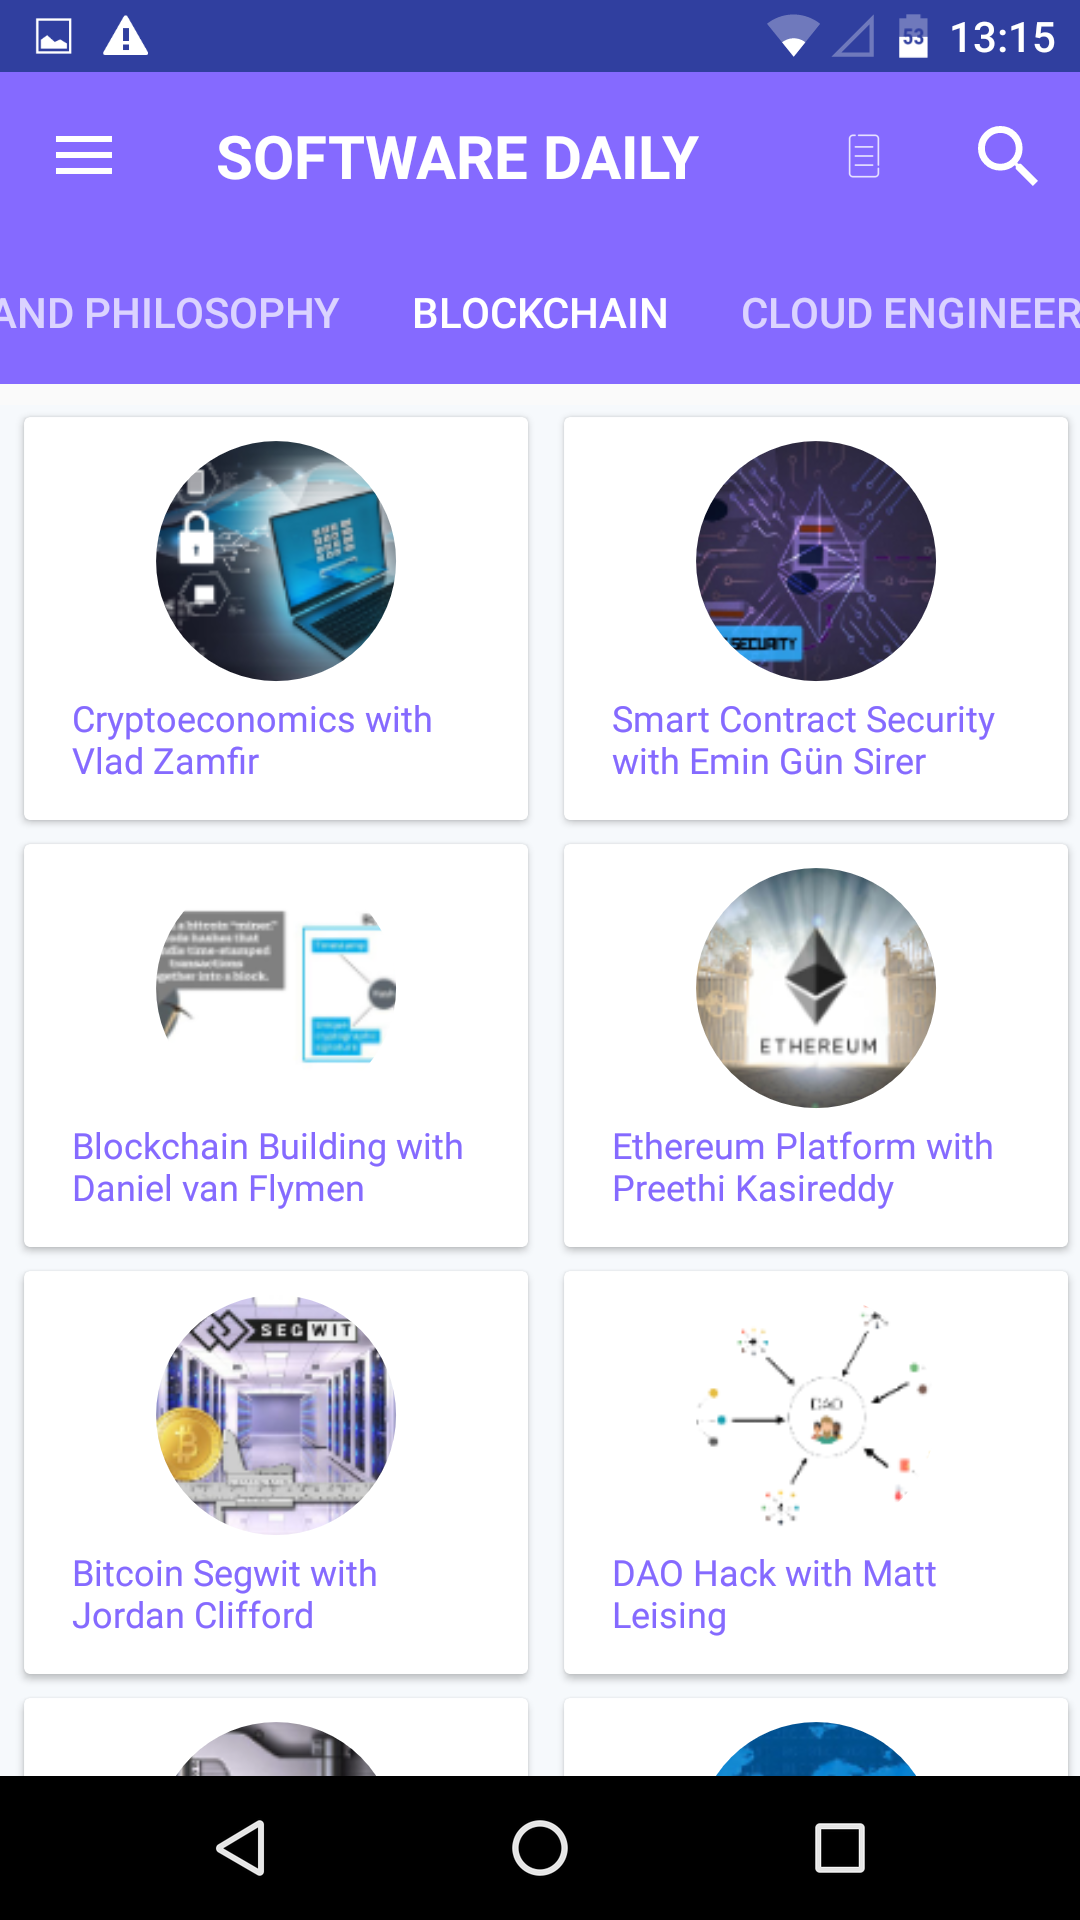
\includegraphics[width=40mm, height=70mm, scale=0.1]{img/before_list_view.png}}
    \column{0.5\textwidth}
    \pause
    \centering{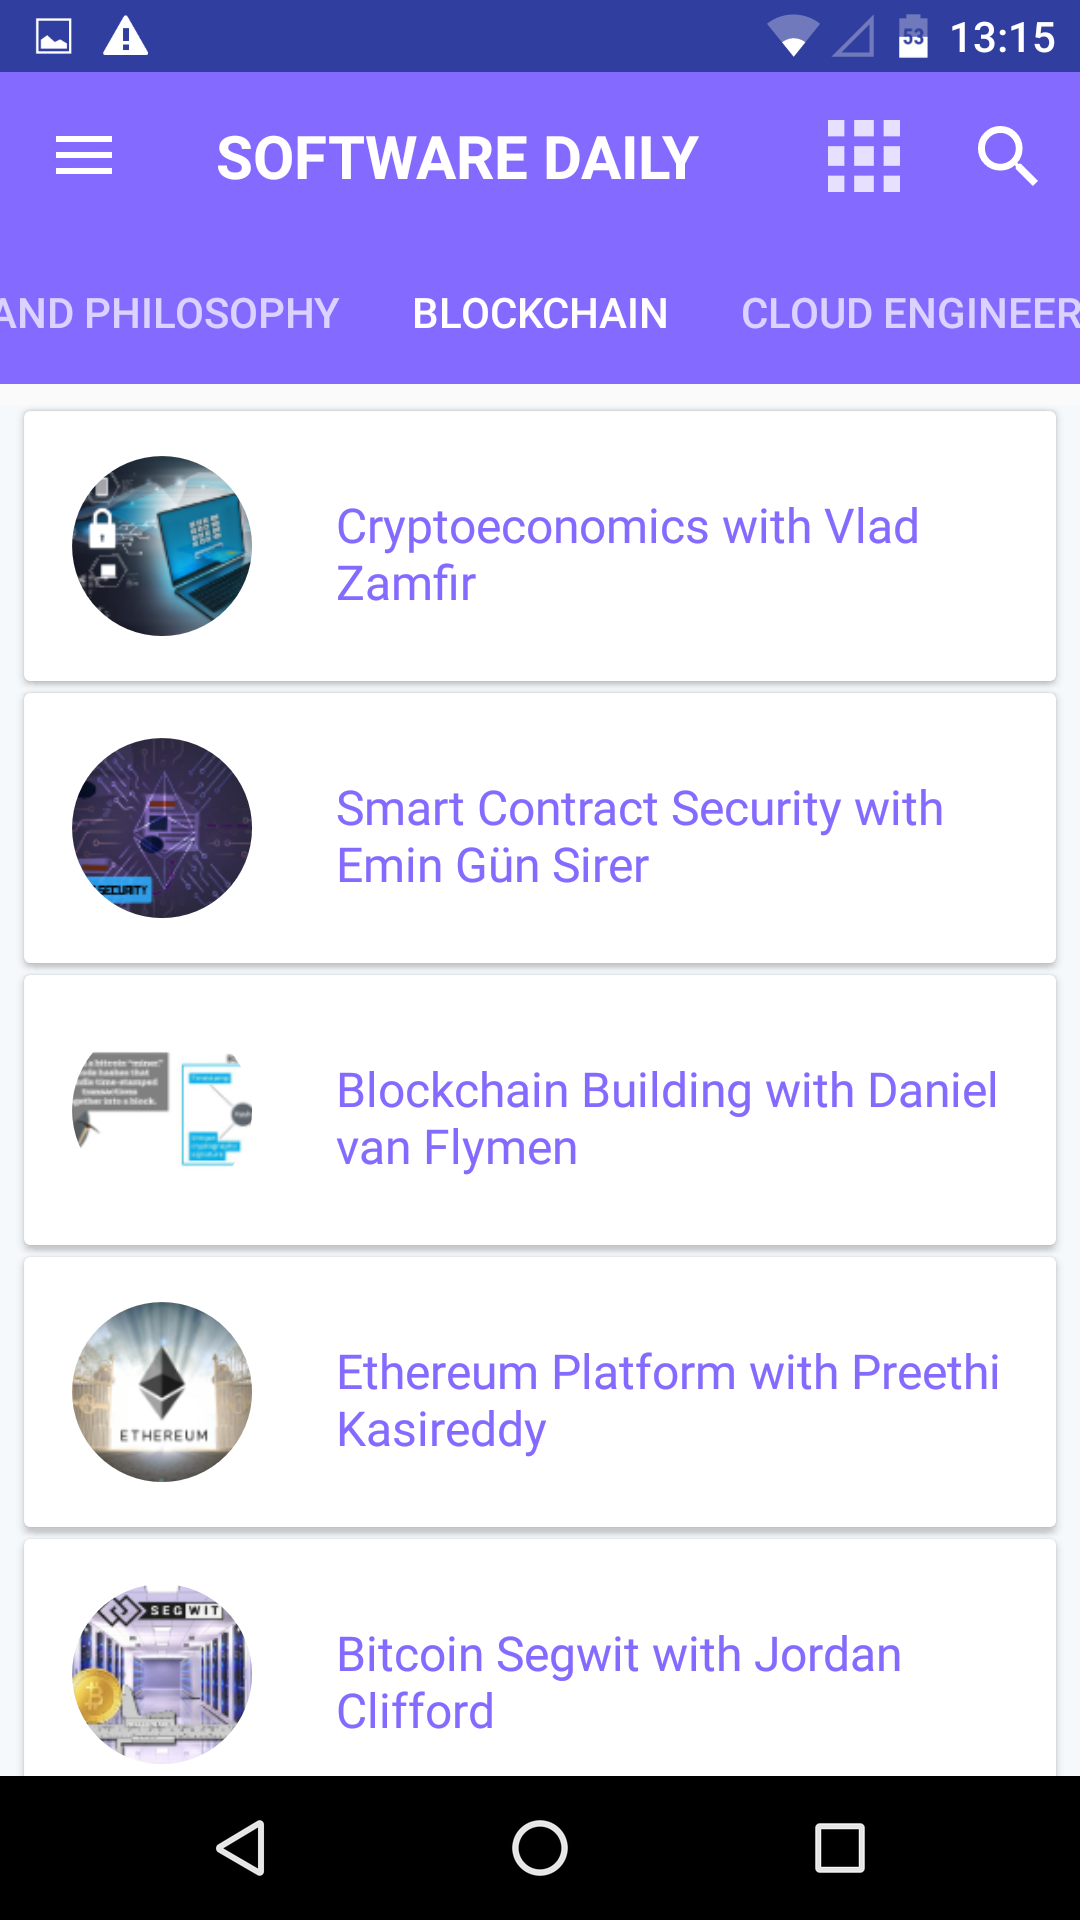
\includegraphics[width=40mm, height=70mm, scale=0.1]{img/after_list_view.png}}
  \end{columns}
\end{frame}

% -------------------------------------

\subsection{feature 2 - resume episode playback}
\begin{frame}{feature 2 - resume episode playback}
  \begin{columns}
    \column{0.7\textwidth}
    \centering{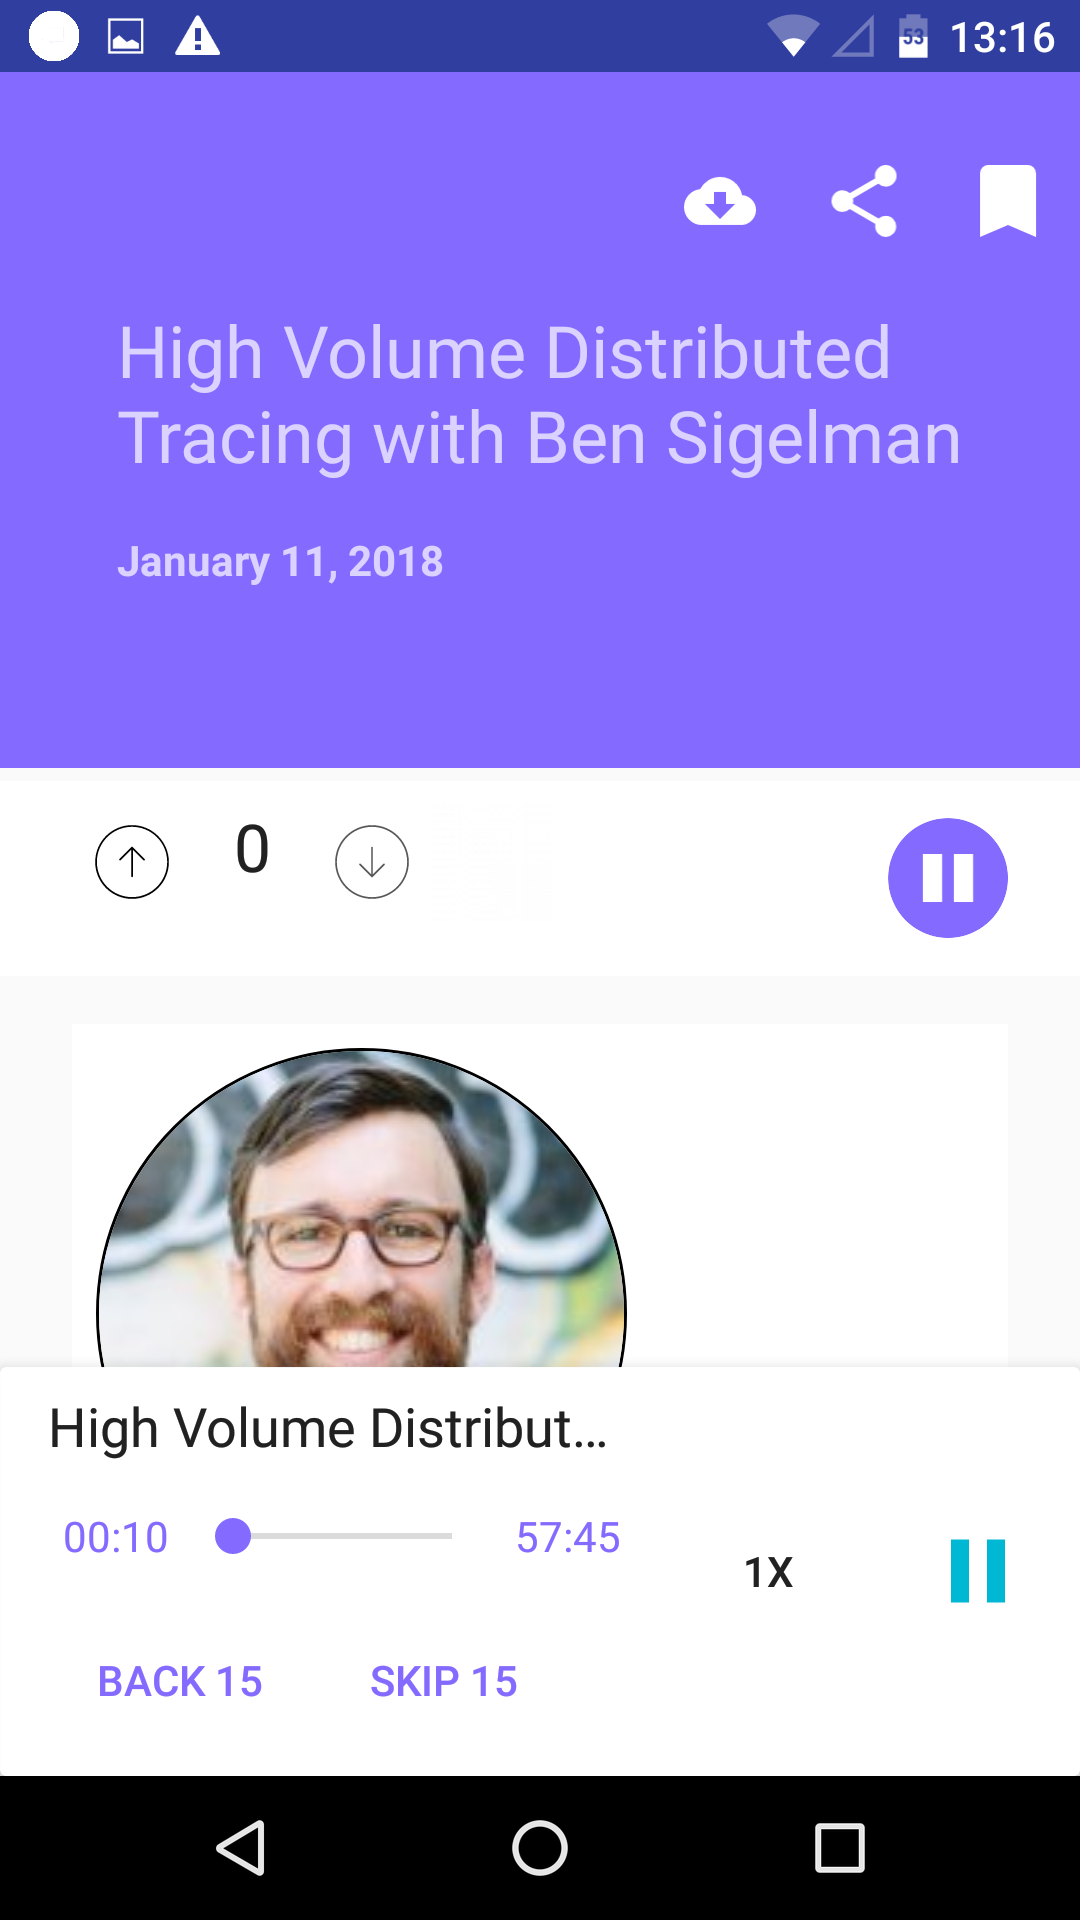
\includegraphics[width=40mm, height=70mm, scale=0.1]{img/before_resume.png}}
    \column{0.4\textwidth}
    \pause
    \centering{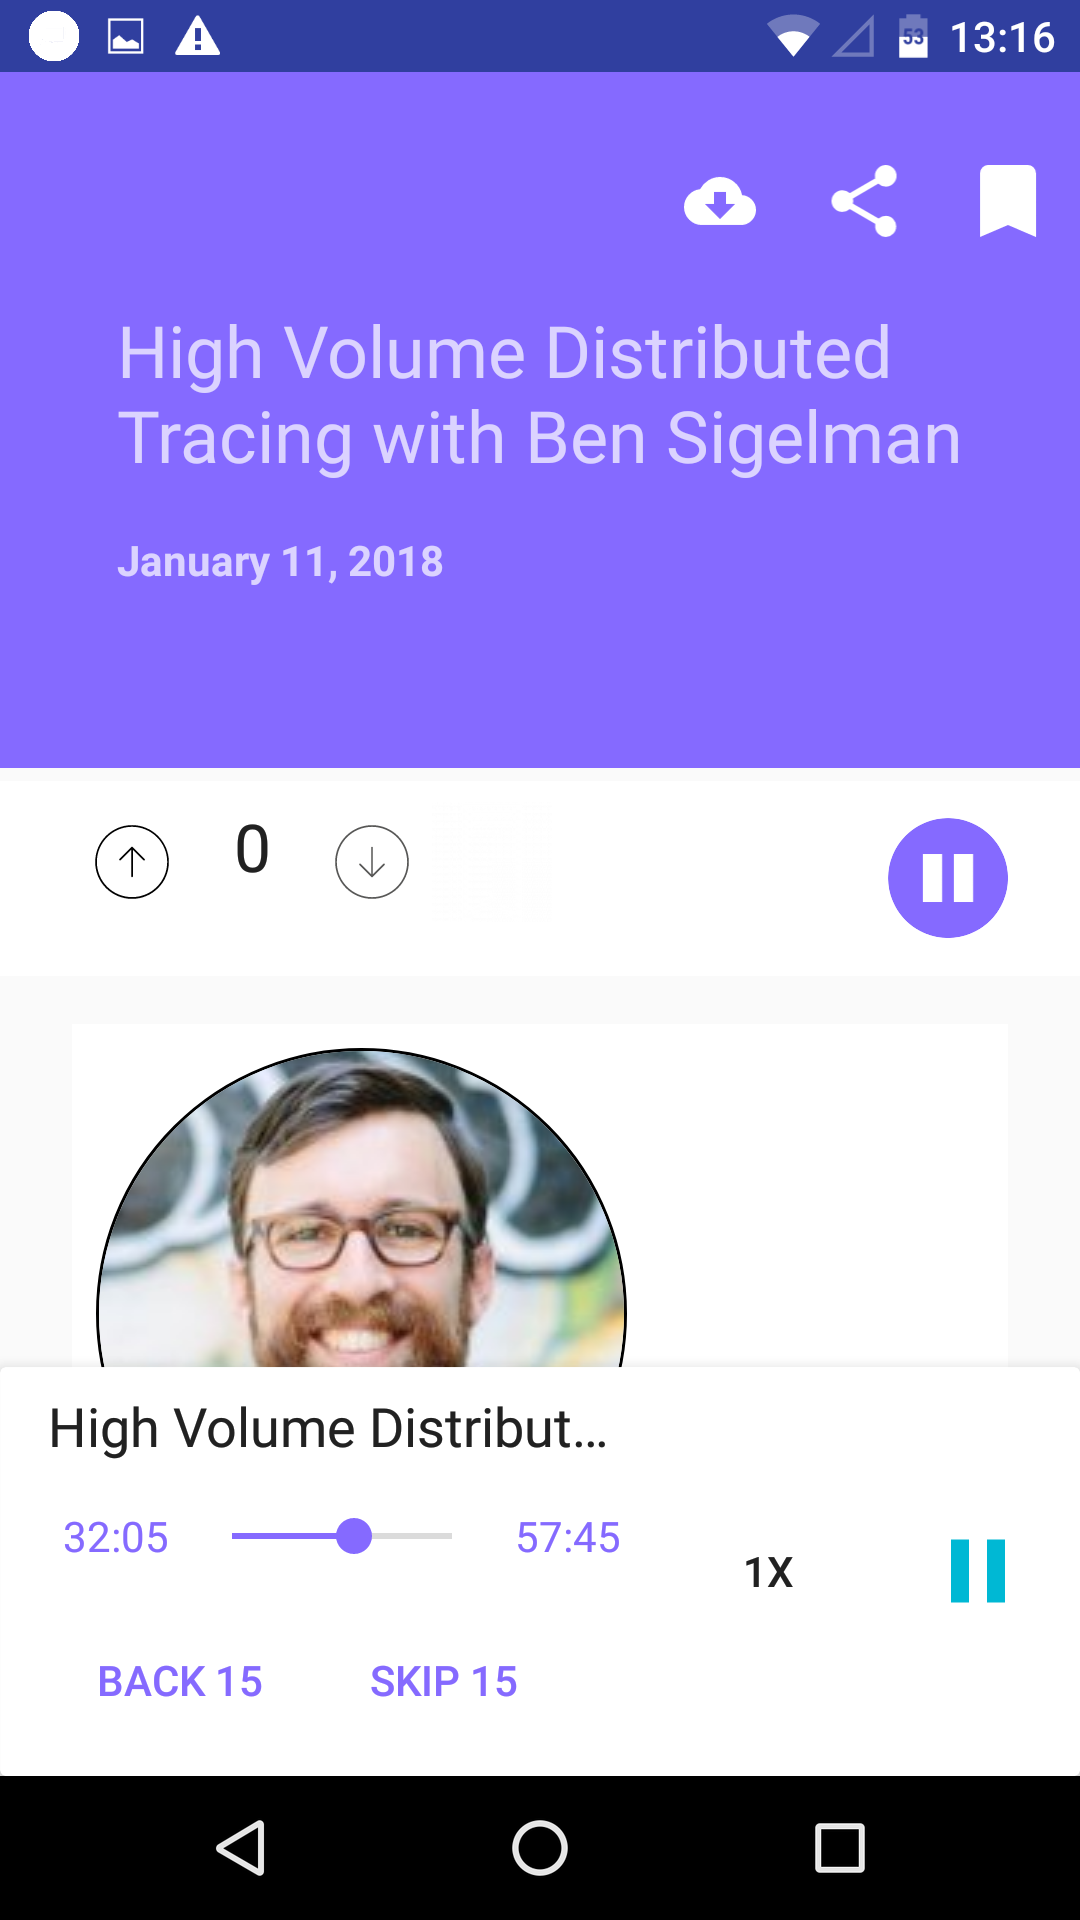
\includegraphics[width=40mm, height=70mm, scale=0.1]{img/after_resume.png}}
  \end{columns}
\end{frame}


\subsection{feature 3 - view downloaded episodes}
\begin{frame}{feature 3 - view downloaded episodes}
  \begin{columns}
    \column{0.7\textwidth}
    \centering{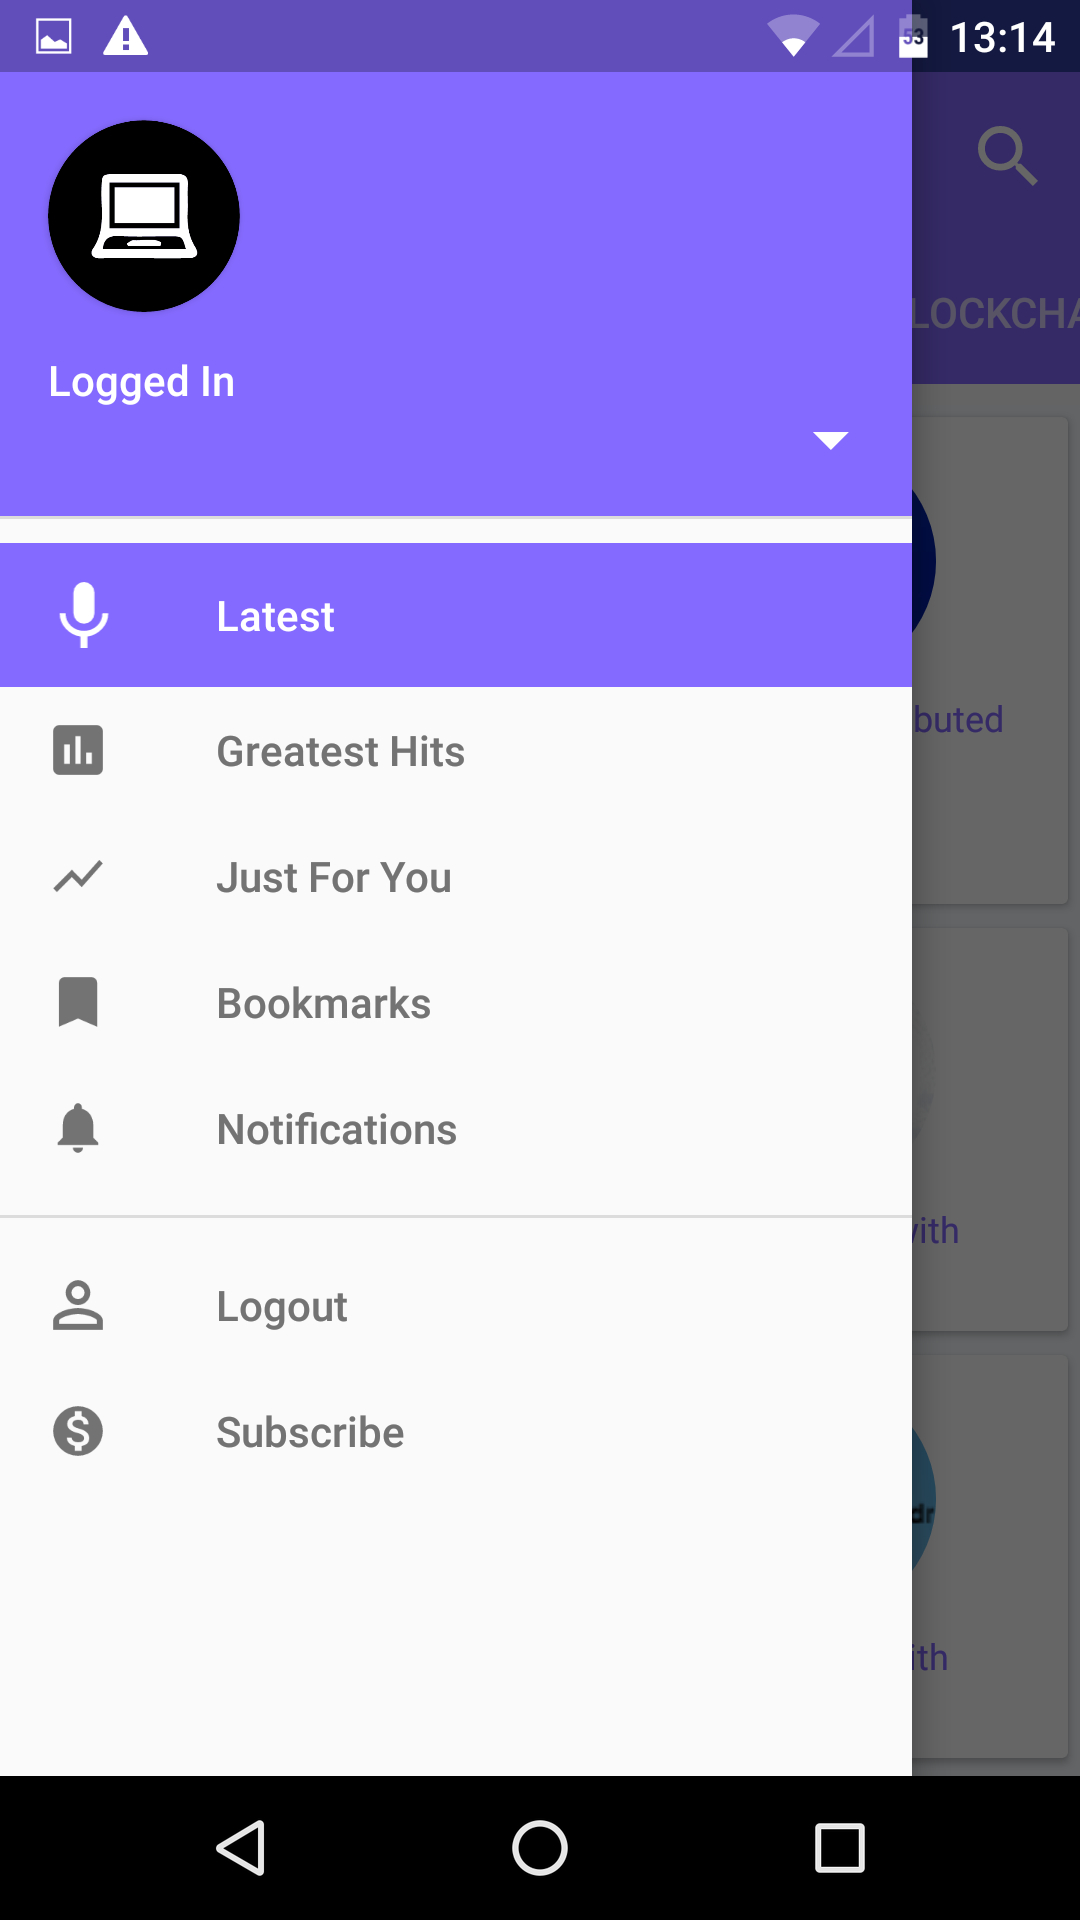
\includegraphics[width=40mm, height=70mm, scale=0.1]{img/bookmarks_menu.png}}
    \column{0.4\textwidth}
    \pause
    \centering{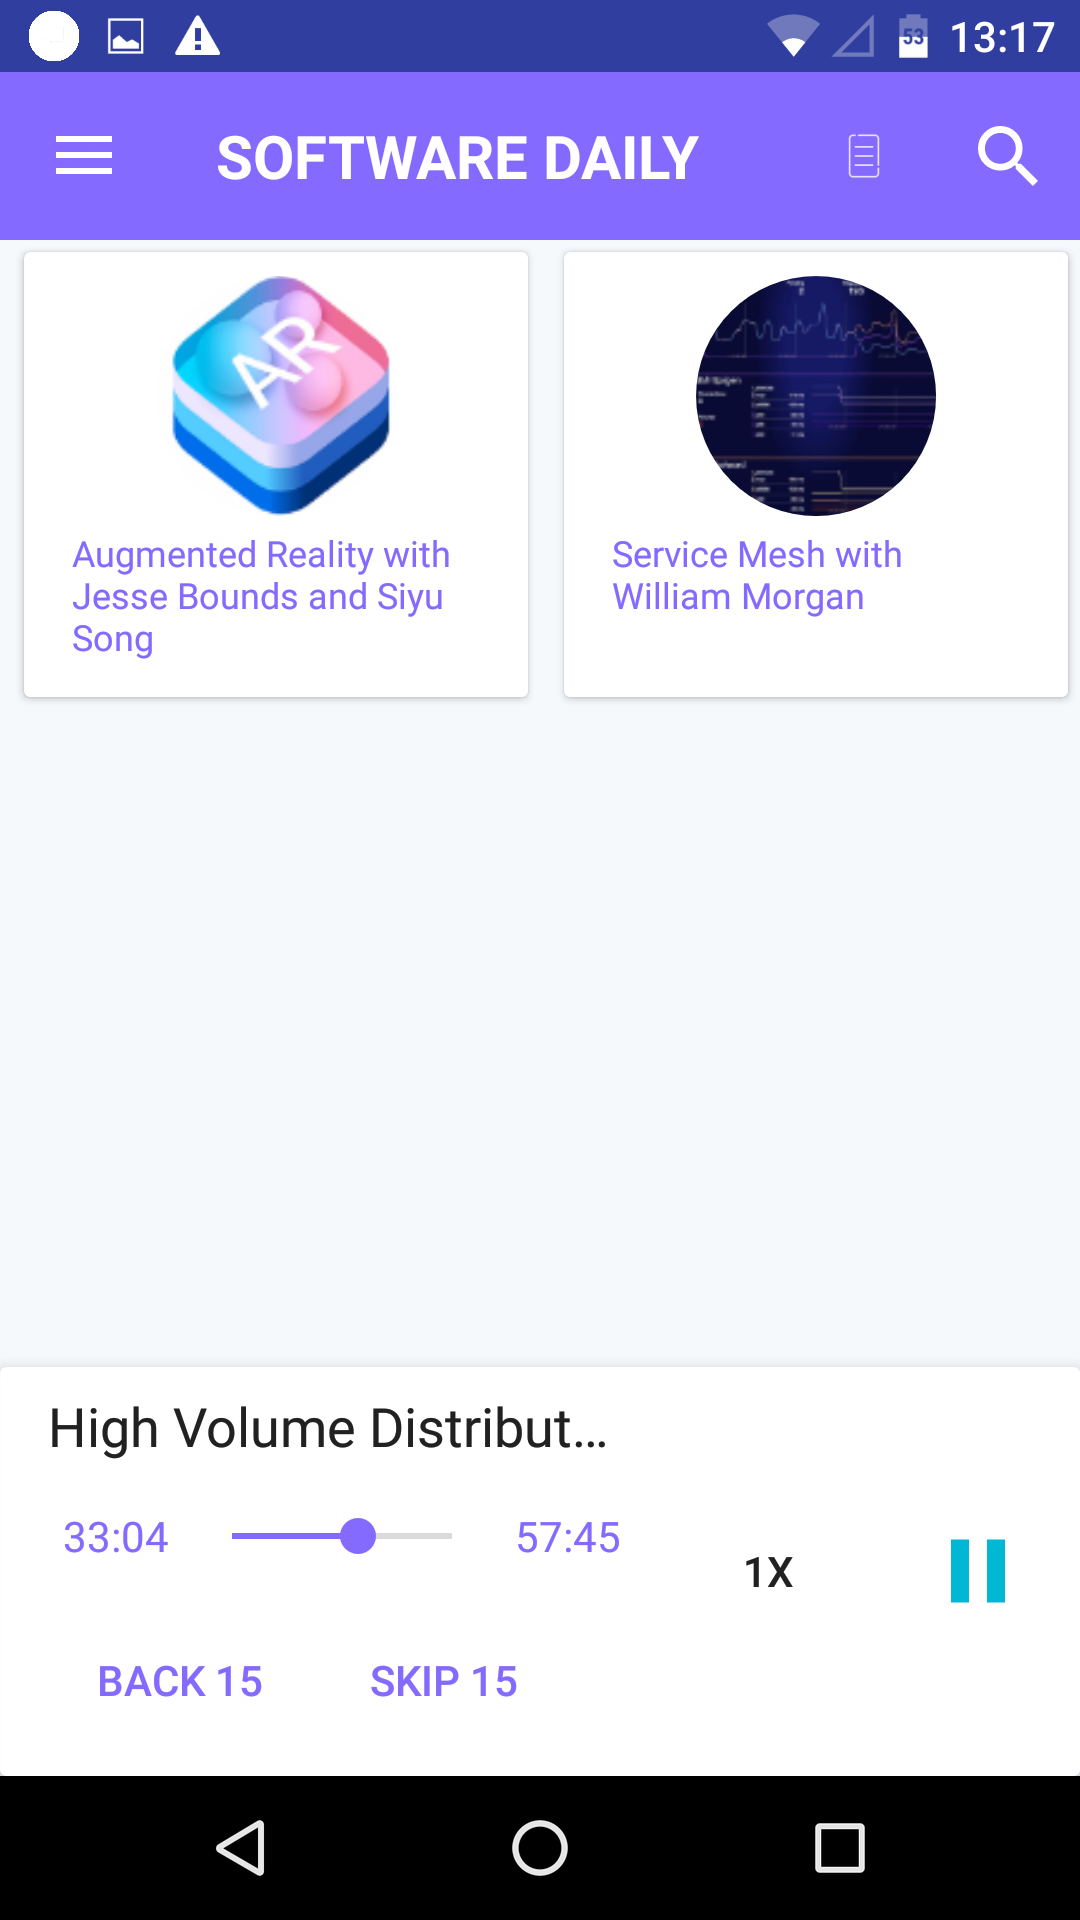
\includegraphics[width=40mm, height=70mm, scale=0.1]{img/dw_episodes.png}}
  \end{columns}
\end{frame}

% -------------------------------------

\subsection{feature 4 - user accounts profile picture}
\begin{frame}{feature 4 - user accounts profile picture}
  \begin{columns}
    \column{0.4\textwidth}
    \centering{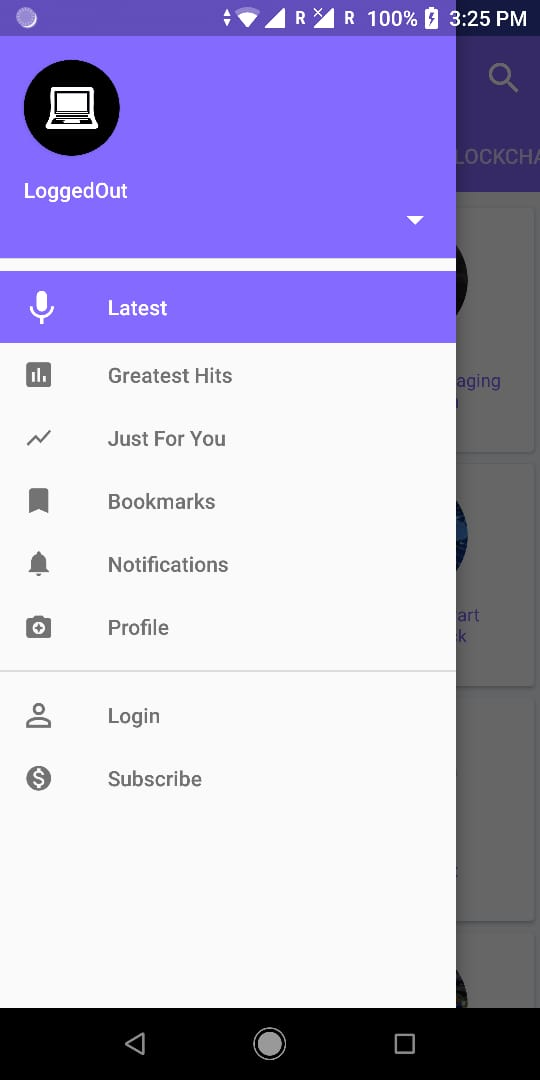
\includegraphics[width=35mm, height=65mm, scale=0.1]{img/profile_menu.jpeg}}
    \column{0.4\textwidth}
    \pause
    \centering{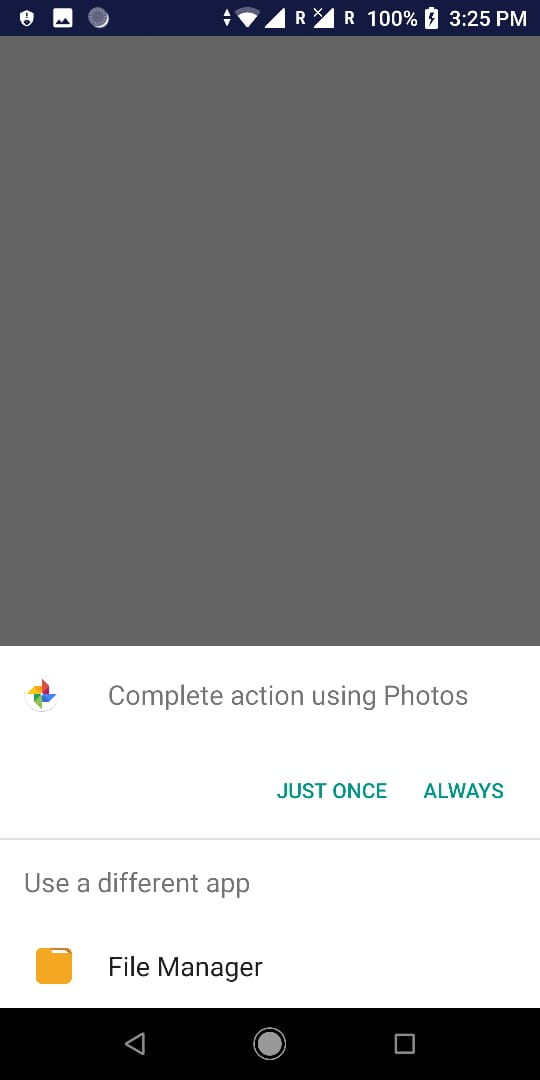
\includegraphics[width=35mm, height=65mm, scale=0.1]{img/com_action.jpeg}}
    \column{0.4\textwidth}
    \pause
    \centering{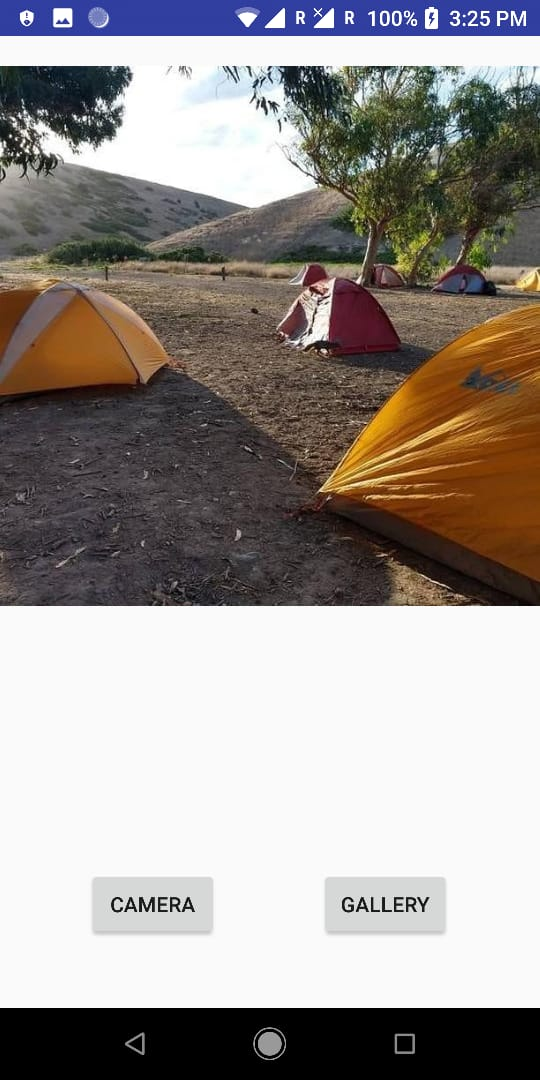
\includegraphics[width=35mm, height=65mm, scale=0.1]{img/profile_pic_set.jpeg}}
  \end{columns}
\end{frame}

% -------------------------------------

\section{}
\begin{frame}{}
  \centering{Thank you! Questions ?}
\end{frame}
\end{document}
%%% Local Variables:
%%% mode: latex
%%% TeX-master: t
%%% End:
